\chapter{Durchführung}

\section{Nichtlineare Optik/ Second Harmonics Generation}
In diesem Teil soll mit einem nichtlinearen Kristall ($\beta$-Bariumborat, "BBO") die zweite Harmonische des Lasers erzeugt werden. Der von uns verwendete Glasfaserlaser besitzt eine zentrale Wellenlänge von $1560\si{\nano\meter}$, die zweite Harmonische ist also bei etwa $780\si{\nano\meter}$ im roten Spektralbereich zu erwarten.
	
Der Versuchsaufbau ist in Abb.\ref{shg_aufbau} schematisch dargestellt.
Zunächst wurde das $\lambda/2$-Plättchen so gedreht, dass der Laserstrahl den Polfilter mit maximaler Intensität passiert, um optimale Bedingungen für die Frequenzverdopplung zu schaffen. Dann wurde die Position des BBO-Kristalls so angepasst, dass er vom Laser genau getroffen wurde. Nach relativ zeitintensiver Justage konnten wir einen roten Laserpunkt auf einem Blatt Papier, das wir hinter dem BBO-Kristall platziert haben erkennen. Nach Entfernen des Blattes und weiterer Feinjustage wurde der frequenzverdoppelte Teil des Laserstrahls durch den dichroitischen Strahlteiler von der Fundamentalen abgespalten und auf einen Schirm geworfen, auf den die Glasfaser unseres Spektroskops gerichtet war. Die Daten des Spektroskops sind in Abb. \ref{shg_spektrum} dargestellt. Das Maximum bei ca. $780\si{\nano\meter}$ ist deutlich zu erkennen und liegt im Rahmen der Erwartungen. Im Vergleich zum spektralen Profil des Laserlichts (siehe Abb. \ref{laserprofil}) fällt auf, dass dieses zwei ausgeprägte lokale Maxima besitzt, während die zweite Harmonische drei aufweist. Dies lässt sich durch die im Kristall vollzogene Faltung des eingestrahlten Laserpulses erklären.


\begin{figure}[H]
	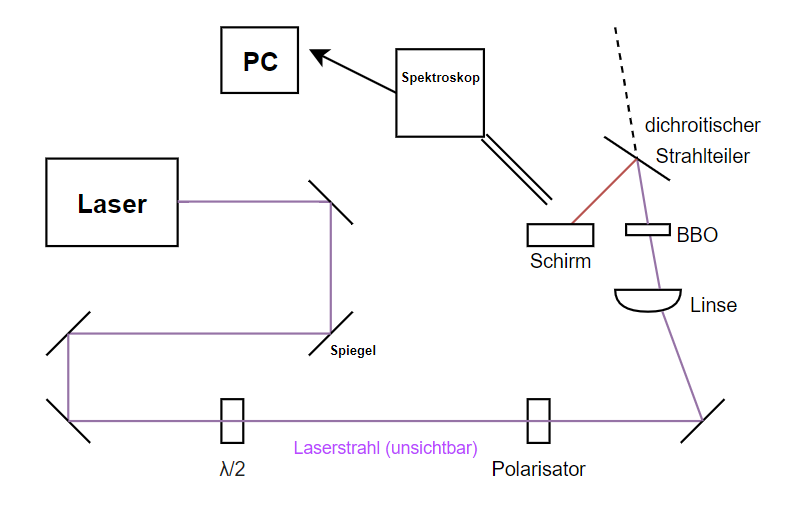
\includegraphics[width=14cm]{Abb/shg_aufbau.png}
	\caption{Schematische Darstellung des Versuchsaufbaus zur Nichtlinearen Optik.}
	\label{shg_aufbau}
\end{figure}
	
\pgfplotsset{width=0.6\textwidth,height=4cm,scale only axis=true}
\begin{figure}
  \centering
  \begin{tikzpicture}
    \begin{axis}[ 
      xmin=720,xmax=840,
      /pgf/number format/1000 sep={},
			xlabel={Wellenlänge [nm]},
			ylabel={Intensität [counts]}
    ]
    \addplot[ 
      color = black,
      mark  = none,
      thick
    ] table
    {Mess/spektrum_shg_max.dat};
		\addlegendentry{Messwerte};
    \end{axis}
  \end{tikzpicture} 
  \caption{Spektrum der zweiten Harmonischen bei voller Intensität des Pumpstrahls. Auffällig sind die drei Maxima in der Frequenzverteilung.}
  \label{shg_spektrum}
\end{figure}



\begin{figure}[H]
	\begin{center}
		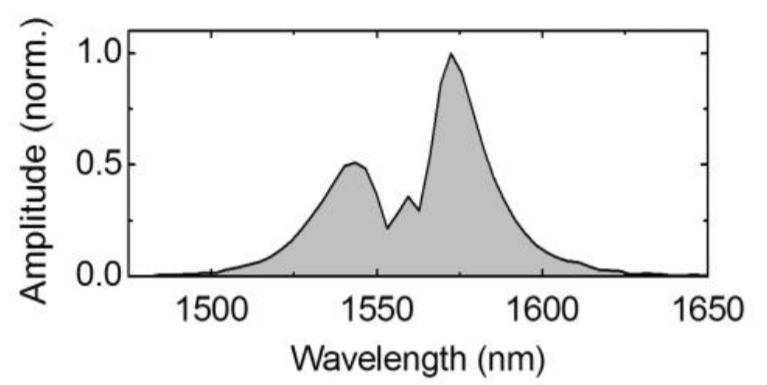
\includegraphics[width=14cm]{Abb/laserprofil.png}
		\caption{Spektrales Profil des eingestrahlten Laserlichts, also der Fundamentalen mit zwei Maxima.}
		\label{laserprofil}
	\end{center}
\end{figure}

Anschließend wurden durch Verdrehen des $\lambda/2$-Plättchens verschiedene Pumpflüsse eingestellt um Intensität der zweiten Harmonischen in Abhängigkeit der Leistung des eingestrahlten Lasers zu untersuchen. Die Ergebnisse sind in Abb. \ref{intensitätmod} zu sehen. Wie zu erwarten zeigt sich ein quadratisches Verhalten der Intensität der second harmonics bezüglich der eingestrahlten Leistung.

\begin{figure}
  \centering
  \begin{tikzpicture}
    \begin{axis}[ 
      %xmin=720,xmax=840,
      /pgf/number format/1000 sep={},
			xlabel={Leistung [mW]},
			ylabel={Intensität [counts]},
			legend pos=north west
    ]
    \addplot[ 
      color = black,
      mark  = x,
      thick
			] table [x=pw,y=int]
    {Mess/shg_int.dat};
		\addlegendentry{Messwerte};
    \end{axis}
  \end{tikzpicture} 
  \caption{Intensität der zweiten Harmonischen in Abhängigkeit des Pumpflusses.}
  \label{intensitätmod}
\end{figure}

%\begin{figure}[H]
%	\begin{center}
%		\includegraphics[width=14cm]{intensmod.png}
%		\caption{Intensität der zweiten Harmonischen in Abhängigkeit des Pumpflusses.}
%		\label{intensitätmod}
%	\end{center}
%\end{figure}


\section{Autokorrelation}
\begin{figure}[H]
	\begin{center}
		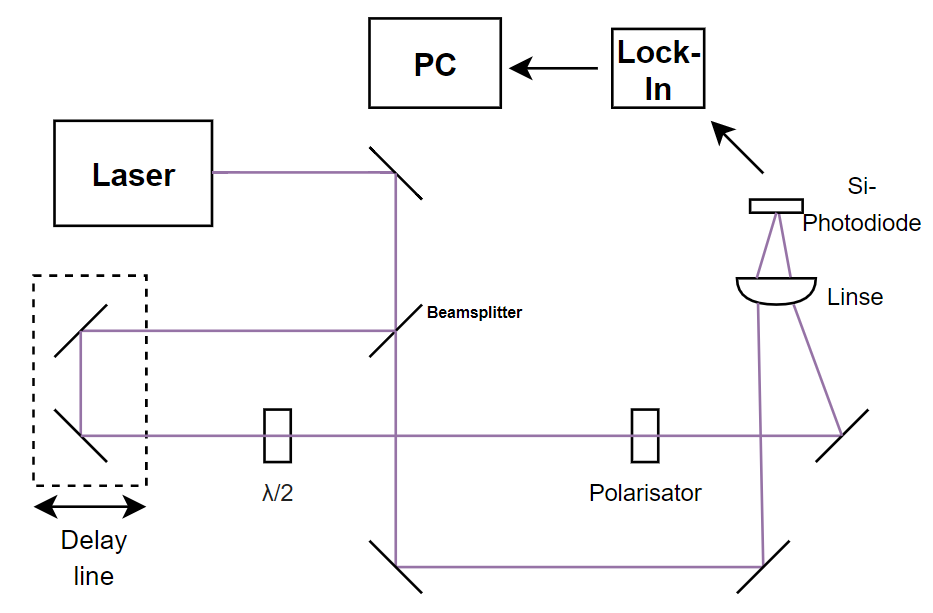
\includegraphics[width=14cm]{Abb/autokorr_aufbau.png}
		\caption{Aufbau des Versuchsteils zur nichtlinearen Autokorrelation}
		\label{autokorr_aufbau}
	\end{center}
\end{figure}

Hier sollte die Impulsdauer des eingestrahlten Laserlichts mittels nichtlinearer Autokorrelation ermittelt werden. Dazu wurden sowohl der Pumpstrahl, welcher über eine bewegliche Delay-Line geführt wurde, als auch der Abtaststrahl so fokussiert, dass sich beide Strahlen auf einer Silizium-Photodiode genau überlagern. Zu Beginn wurde mithilfe von $\lambda/2$-Plättchen und Polarisator im Pumpstrahl die gleiche Intensität wie im Abtaststrahl eingestellt. Das Signal der Photodiode wurde in Abhängigkeit zur Verzögerungszeit der Delay-Line gemessen und zunächst von einem Lock-In-Verstärker aufbereitet und dann in ein LabView-Programm am PC gespeist, das die Autokorrelationskurve plottet. Der Aufbau dieses Versuchsteils ist in Abb. \ref{autokorr_aufbau} schematisch dargestellt.
Das Autokorrelationssignal konnte bei einer Verzögerungszeit von ca. $52 \si{\pico\second}$ gefunden werden. Wir nehmen an, dass die Laserpulse ein gaußförmiges Intensitäts-Zeit-Profil aufweisen, wodurch die Korrelationskurve ebenfalls gaußförmig ausfallen wird (Autokorrelation einer Gaußkurve ergibt wieder eine Gaußkurve). Der Gaußfit bestätigt unsere Vermutung (siehe Abb. \ref{autokorr_normal}) und nennt für die Standardabweichung einen Wert von $\sigma=38,7\si{\femto\second}$. Damit kann die full duration at half maximum (FDHM) ermittelt werden:

Ohne Beschränkung der Allgemeinheit kann zunächst von einer zentrierten Gaußfunktion ausgegangen werden, da eine Verschiebung die FDHM nicht verändert:

\[g_{0,\sigma^2}(x)=\dfrac{1}{\sqrt{2\pi\sigma^2}}e^{\dfrac{-x^2}{2\sigma^2}}\]
welche ihr Maximum bei $x=0$ mit $g_{0,\sigma^2}(x=0)=\dfrac{1}{\sqrt{2\pi\sigma^2}}$ annimmt. Die FDHM ist also $|x_{2}-x_{1}|$ mit $g_{0,\sigma^2}(x_{1})=g_{0,\sigma^2}(x_{2})=\dfrac{1}{2\sqrt{2\pi\sigma^2}}$

Berechnung von $x_{1,2}$:
\begin{align*}
\dfrac{1}{2\sqrt{2\pi\sigma^2}}&=\dfrac{1}{\sqrt{2\pi\sigma^2}}e^{\dfrac{-x^2}{2\sigma^2}}\\
\dfrac{1}{2}&=e^{\dfrac{-x^2}{2\sigma^2}}\\
ln\Big(\dfrac{1}{2}\Big)&=\dfrac{-x^2}{2\sigma^2}\\
2\sigma^2ln\Big(\dfrac{1}{2}\Big)&=-x^2\\
x_{1,2}&=\pm\sqrt{2ln(2)}\sigma\\
\Rightarrow \text{FDHM}&=2\sqrt{2ln(2)}\sigma\approx2,355\sigma
\end{align*}

Da die Gaußfunktion reellwertig und symmetrisch ist, ist die Autokorrelation identisch mit der Faltung der Gaußkurve mit sich selbst. Hierfür gilt $g_{0,\tilde{\sigma}^2} \ast g_{0,\tilde{\sigma}^2} = g_{0,2\tilde{\sigma}^2}$, wobei $\sigma^2=2\tilde{\sigma}^2 \Leftrightarrow \tilde{\sigma}=\dfrac{1}{\sqrt{2}}\sigma$, wobei im vorliegenden Fall $\sigma$ für die Standardabweichung der Gaußverteilung des Autokorrelationssignals steht und $\tilde{\sigma}$ für die Standardabweichung des ursprünglichen Laserpulses. Die FDHM des Laserpulses ergibt sich nach obigen Betrachtungen zu \[\textbf{FDHM}\approx2,355\tilde{\sigma}=2,355\dfrac{1}{\sqrt{2}}\sigma=2,355\dfrac{1}{\sqrt{2}}\cdot 38,7\si{\femto\second}= \textbf{64,4fs}\]

Dieser Wert weicht um $\dfrac{64,4\si{\femto\second}-50\si{\femto\second}}{50\si{\femto\second}}=28,8\%$ von der Erwartung ($50\si{\femto\second}$) ab, was sich möglicherweise dadurch erklären lässt, dass obige Überlegungen zur Berechnung der FDHM nur gelten, wenn es sich um eine exakte Autokorrelation handelt, der Pumppuls und der Abtastpuls also genau die gleiche Intensität aufweisen, was mit unseren Mitteln nicht eindeutig ein- bzw. festzustellen war.

Bei der Verwendung einer GaAs-Probe (vor dem Beamsplitter) erhalten wir eine Standardabweichung von $\sigma=64,3\si{\femto\second}$ und damit eine FDHM (bezüglich $\tilde{\sigma}$) von $107,1\si{\femto\second}$. Das Signal ist in Abb. \ref{autokorr_gaas} dargestellt. Die höhere FDHM lässt sich dadurch erklären, dass GaAs ein dispersives Medium und der Laserpuls relativ breitbandig, also nicht monochromatisch, ist. Dadurch durchlaufen die verschiedenen Wellenlängen die Probe mit unterschiedlicher Geschwindigkeit, was zu einer Verbreiterung des Pulses führt.

\begin{figure}
  \centering
  \begin{tikzpicture}
    \begin{axis}[
			xlabel={Verzögerung [ps]},
			ylabel={Intensität, relativ},
      xmin=51.5,xmax=53,
      /pgf/number format/1000 sep={}
    ]
    \addplot[ 
      color = black,
      mark  = none,
      thick
    ] table [
				x=verz,y=int,
				y expr=\thisrow{int}/(8.533540E-3)
			]
    {Mess/autokorr/lockin_ch0_x.dat};
		\addlegendentry{Messwerte};
		\addplot[
		  color = blue,
			mark  = none,
	    thick,
			domain=52.1:52.35
			]%
						{1+(exp((-(x-52.2278)^2)/(2*0.0387763^2)))*0.93};
		\addlegendentry{Gaussfit}
		\addplot[mark=none,color=black] coordinates {(52.2278-2.355/2*0.0387763,1.465) (52.2278+2.355/2*0.0387763,1.465)};
		\node[] at (axis cs: 52.4,1.465) {$2.355\sigma$};
    \end{axis}
  \end{tikzpicture} 
  \caption{Autokorrelationssignal mit einer FDHM von $2,355\sigma=2,355\cdot 38,7\si{\femto\second}=91,1\si{\femto\second}$}
  \label{autokorr_normal}
\end{figure}



%\begin{figure}[H]
%	\begin{center}
%		\includegraphics[width=14cm]{autokorr_normal.png}
%		\caption{Autokorrelationssignal mit einer FDHM von $2,355\sigma=2,355\cdot 38,7\si{\femto\second}=91,1\si{\femto\second}$}
%		\label{autokorr_normal}
%	\end{center}
%\end{figure}

\begin{figure}
  \centering
  \begin{tikzpicture}
    \begin{axis}[
			xlabel={Verzögerung [ps]},
			ylabel={Intensität, relativ},
      xmin=51.5,xmax=53,
      /pgf/number format/1000 sep={}
    ]
    \addplot[ 
      color = black,
      mark  = none,
      thick
    ] table [
				x=verz,y=int,
				y expr=\thisrow{int}/(3.646630E-4)
			]
    {Mess/autokorr_gaas/lockin_ch0_x.dat};
		\addlegendentry{Messwerte};
    \addplot[
		  color = blue,
			mark  = none,
	    thick,
			domain=51.95:52.5
			]%
			{1+(exp((-(x-52.237)^2)/(2*0.0643781^2)))*1.87};
			\addlegendentry{Gaussfit};
      \addplot[mark=none,color=black] coordinates {(52.237-2.355/2*0.0643781,1.93490) (52.237+2.355/2*0.0643781,1.93490)};
      \node[] at (axis cs: 52.45,1.93490) {2.355$\,\sigma$};
    \end{axis}
  \end{tikzpicture} 
  \caption{Autokorrelationssignal (mit GaAs-Probe) mit einer FDHM von $2,355\sigma=2,355\cdot 64,3\si{\femto\second}=151,4\si{\femto\second}$}
  \label{autokorr_gaas}
\end{figure}
	
%\begin{figure}[H]
%	\begin{center}
%		\includegraphics[width=14cm]{autokorr_gaas}
%		\caption{Autokorrelationssignal (mit GaAs-Probe) mit einer FDHM von $2,355\sigma=2,355\cdot 64,3\si{\femto\second}=151,4\si{\femto\second}$}
%		\label{autokorr_gaas}
%	\end{center}
%\end{figure}
	
\section{Ladungsträgerdynamik in InGaAs}	
In diesem Versuchsteil sollte die Ladungsträgerdynamik in InGaAs mittels eines Pump-Probe-Versuchs herausgearbeitet werden. Dazu wurde eine GaAs Probe so in den Strahlengang eingebaut, dass sich Pump- und Abtaststrahl genau im Kristall kreuzen. Der Pumpstrahl wurde dann abgeblockt und der Abtaststrahl mittels InGaAs-Photodiode, Lock-In Verstärker und PC ausgewertet. Der Aufbau des Pump-Probe Versuchs ist in Abb. \ref{pp_aufbau} zu sehen.

\begin{figure}[h]
	\begin{center}
		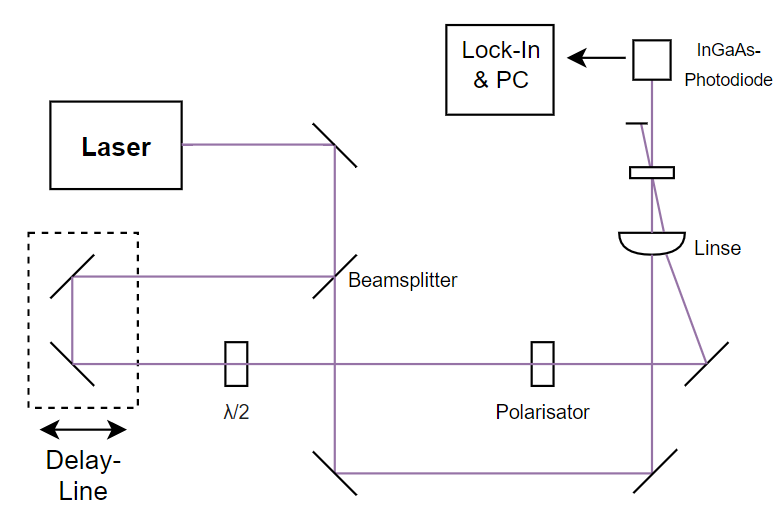
\includegraphics[width=14cm]{Abb/pumpprobe_aufbau.png}
		\caption{Aufbau des Pump-Probe Versuchs}
		\label{pp_aufbau}
	\end{center}
\end{figure}

Um die Ladungsträgerdynamik zu visualisieren wurde die Intensität des Abtaststrahls gegen die Verzögerung des Pumpstrahls aufgetragen. Das Diagramm ist in Abb. \ref{zerfall} zu sehen. Man erkennt deutlich zwei verschiedene Abfälle des Graphen: zunächst einen mit einer hohen Abklingkonstante an den sich ein deutlich langsamerer Zerfall anschließt. Beide Abschnitte des Graphen können gut mit einer Exponentialfunktion gefittet werden. Als $1/e$-Abklingkonstante erhalten wir beim Fit für den schnellen Zerfall $\tau=1,38\si{\pico\second}$ und für den langsamen $\tau=177,6\si{\pico\second}$. 

Schließlich haben wir noch die Maximalintensität des Abtaststrahls (also das Maximum der Kurven analog zu Abb. \ref{zerfall}) bei verschiedenen Pumpflüssen von 10 bis 65mW aufgenommen und graphisch dargestellt (siehe Abb. \ref{int_leistung} ). Wir hatten hier einen linearen Zusammenhang erwartet, da die Zahl der durch den Pumpstrahl angeregten Ladungsträger linear zu dessen Intensität ist. Wir erhalten immerhin einen monoton steigenden Zusammenhang, jedoch lässt die Linearität zu wünschen übrig. Als mögliche Fehlerquelle sei zu nennen, dass die Maximalintensität des Abtaststrahls ein sehr scharfer Peak ist und unsere Schritte für die Verzögerungszeit eventuell zu groß gewählt waren um den wahren Maximalwert zuverlässig zu messen.

%\begin{figure}[h]
%	\begin{center}
%		\includegraphics[width=14cm]{zerfall.png}
%		\caption{Ladungsträgerdynamik von InGaAs}
%		\label{zerfall}
%	\end{center}
%\end{figure}
%
%\begin{figure}[h]
%	\begin{center}
%		\includegraphics[width=14cm]{int_leistung.png}
%		\caption{Zusammenhang der Abtastintensität zum Pumpfluss. Hier wäre ein linearer Zusammenhang erwartet worden.}
%		\label{int_leistung}
%	\end{center}
%\end{figure}

\begin{figure}
  \centering
  \begin{tikzpicture}
    \begin{axis}[
			xlabel={Verzögerung [ps]},
			ylabel={Intensität [counts]},
      xmin=25,xmax=200,
      /pgf/number format/1000 sep={}
    ]
    \addplot[ 
      color = black,
      mark  = none,
      thick
    ] table [
				x=verz,y=int,
				%y expr=\thisrow{int}/(3.646630E-4)
			]
    {Mess/InGaAs_max/lockin_ch0_x.dat};
		\addlegendentry{Messwerte}
    \addplot[
		  color = blue,
			mark  = none,
	    thick,
			domain=50:70
			]%
			{0.229443*exp(-(x-50.4365)/1.37512)+0.201598};
	  \addlegendentry{Exp. Fit};
    \addplot[
		  color = red,
			mark  = none,
	    thick,
			domain=63:200
			]%
			{0.253803*exp(-(x-32.2308)/177.599)-0.0149594};
     \addlegendentry{Exp. Fit};
    \end{axis}
  \end{tikzpicture} 
  \caption{Ladungsträgerdynamik von InGaAs}
  \label{zerfall}
\end{figure}

\begin{figure}
  \centering
  \begin{tikzpicture}
    \begin{axis}[ 
      %xmin=720,xmax=840,
      /pgf/number format/1000 sep={},
			xlabel={Leistung [mW]},
			ylabel={Intensität [counts]},
			legend pos=north west
    ]
    \addplot[ 
      color = black,
      mark  = x,
      thick
			] table 
    {Mess/InGaAs_Int.dat};
		\addlegendentry{Messwerte};
    \end{axis}
  \end{tikzpicture} 
  \caption{Zusammenhang der Abtastintensität zum Pumpfluss. Hier wäre ein linearer Zusammenhang erwartet worden.}
  \label{int_leistung}
\end{figure}

